\documentclass{beamer}

% Should be documentclass beamer

\mode<presentation>
{
%  \usetheme[hideothersubsections]{PaloAlto}
  \usetheme{metropolis}
  \setbeamercovered{transparent}
}

\input{commonm}

\newcommand{\hdr}[2]{
  \title[CS 5220, Fall 2017]{CS 5220: #2}
  \author{David Bindel}
  \institute{Cornell}
  \date{#1}
}


\hdr{2017-10-19}{Dense Linear Algebra}

\begin{document}

\begin{frame}
  \titlepage
\end{frame}


\begin{frame}
  \frametitle{Parallel matmul}

  \begin{itemize}
  \item Basic operation: $C = C+AB$
  \item Computation: $2n^3$ flops
  \item Goal: $2n^3/p$ flops per processor, minimal communication
  \item Two main contenders: SUMMA and Cannon
  \end{itemize}
\end{frame}



\begin{frame}[fragile]
  \frametitle{Outer product algorithm}

  Serial: Recall outer product organization:
\begin{lstlisting}
for k = 0:s-1
  C += A(:,k)*B(k,:);
end
\end{lstlisting}

  \vspace{5mm}
  Parallel: Assume $p = s^2$ processors, block $s \times s$ matrices. \\
  For a $2 \times 2$ example:
  \[
  \begin{bmatrix}
    C_{00} & C_{01} \\
    C_{10} & C_{11}
  \end{bmatrix} =
  \begin{bmatrix}
    A_{00} B_{00} & A_{00} B_{01} \\
    A_{10} B_{00} & A_{10} B_{01} 
  \end{bmatrix} +
  \begin{bmatrix}
    A_{01} B_{10} & A_{01} B_{11} \\
    A_{11} B_{10} & A_{11} B_{11} 
  \end{bmatrix}
  \]

\begin{itemize}
\item
  Processor for each $(i,j)$ $\implies$ parallel work for each $k$!
\item
  Note everyone in row $i$ uses $A(i,k)$ at once, \\
  and everyone in row $j$ uses $B(k,j)$ at once.
\end{itemize}

\end{frame}


\begin{frame}[fragile]
  \frametitle{Parallel outer product (SUMMA)}

\begin{lstlisting}
for k = 0:s-1
  for each i in parallel
    broadcast A(i,k) to row
  for each j in parallel
    broadcast A(k,j) to col
  On processor (i,j), C(i,j) += A(i,k)*B(k,j);
end
\end{lstlisting}
If we have tree along each row/column, then
\begin{itemize}
\item $\log(s)$ messages per broadcast
\item $\alpha + \beta n^2/s^2$ per message
\item $2 \log(s) (\alpha s + \beta n^2/s)$ total communication 
\item Compare to 1D ring: $(p-1) \alpha + (1-1/p) n^2 \beta$
\end{itemize}

\vspace{2mm}
Note: Same ideas work with block size $b < n/s$

\end{frame}


\begin{frame}
  \frametitle{SUMMA}

  \begin{center}
    \begin{tikzpicture}[scale=2]
      \draw (0,0) rectangle (0.8,0.8);
      \draw (1,0) rectangle (1.8,0.8);
      \draw (2,0) rectangle (2.8,0.8);
      \draw (0,1) rectangle (0.8,1.8);
      \draw (1,1) rectangle (1.8,1.8);
      \draw (2,1) rectangle (2.8,1.8);
      \draw (0,2) rectangle (0.8,2.8);
      \draw (1,2) rectangle (1.8,2.8);
      \draw (2,2) rectangle (2.8,2.8);      
    \end{tikzpicture}
  \end{center}
\end{frame}


\begin{frame}
  \frametitle{SUMMA}

  \begin{center}
    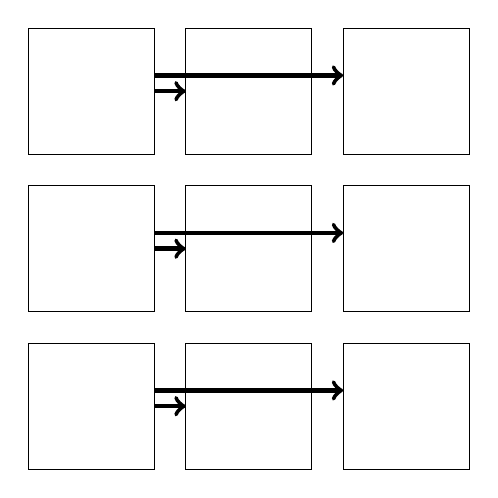
\begin{tikzpicture}[scale=2]
      \draw (0,0) rectangle (0.8,0.8);
      \draw (1,0) rectangle (1.8,0.8);
      \draw (2,0) rectangle (2.8,0.8);
      \draw (0,1) rectangle (0.8,1.8);
      \draw (1,1) rectangle (1.8,1.8);
      \draw (2,1) rectangle (2.8,1.8);
      \draw (0,2) rectangle (0.8,2.8);
      \draw (1,2) rectangle (1.8,2.8);
      \draw (2,2) rectangle (2.8,2.8);
      \draw [ultra thick,->] (0.8,0.4) -- (1,0.4);
      \draw [ultra thick,->] (0.8,0.5) -- (2,0.5);
      \draw [ultra thick,->] (0.8,1.4) -- (1,1.4);
      \draw [ultra thick,->] (0.8,1.5) -- (2,1.5);
      \draw [ultra thick,->] (0.8,2.4) -- (1,2.4);
      \draw [ultra thick,->] (0.8,2.5) -- (2,2.5);
    \end{tikzpicture}
  \end{center}
\end{frame}


\begin{frame}
  \frametitle{SUMMA}

  \begin{center}
    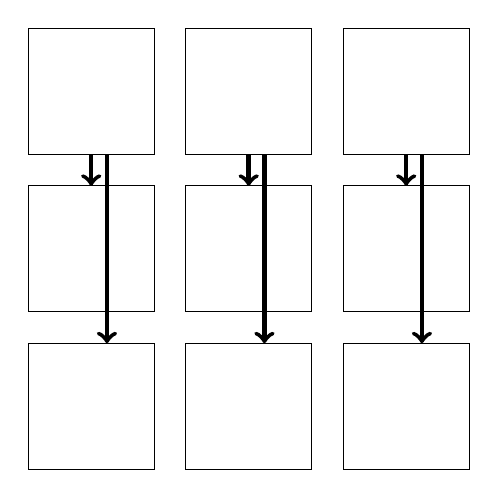
\begin{tikzpicture}[scale=2]
      \draw (0,0) rectangle (0.8,0.8);
      \draw (1,0) rectangle (1.8,0.8);
      \draw (2,0) rectangle (2.8,0.8);
      \draw (0,1) rectangle (0.8,1.8);
      \draw (1,1) rectangle (1.8,1.8);
      \draw (2,1) rectangle (2.8,1.8);
      \draw (0,2) rectangle (0.8,2.8);
      \draw (1,2) rectangle (1.8,2.8);
      \draw (2,2) rectangle (2.8,2.8);
      \draw [ultra thick,->] (0.4,2) -- (0.4,1.8);
      \draw [ultra thick,->] (0.5,2) -- (0.5,0.8);
      \draw [ultra thick,->] (1.4,2) -- (1.4,1.8);
      \draw [ultra thick,->] (1.5,2) -- (1.5,0.8);
      \draw [ultra thick,->] (2.4,2) -- (2.4,1.8);
      \draw [ultra thick,->] (2.5,2) -- (2.5,0.8);
    \end{tikzpicture}
  \end{center}
\end{frame}


\begin{frame}[fragile]
  \frametitle{Parallel outer product (SUMMA)}

If we have tree along each row/column, then
\begin{itemize}
\item $\log(s)$ messages per broadcast
\item $\alpha + \beta n^2/s^2$ per message
\item $2 \log(s) (\alpha s + \beta n^2/s)$ total communication 
\end{itemize}

\vspace{5mm}
Assuming communication and computation can potentially overlap 
{\em completely}, what does the speedup curve look like?

\end{frame}


\begin{frame}
  \frametitle{Reminder: Why matrix multiply?}

  \begin{center}
    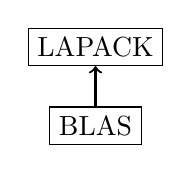
\begin{tikzpicture}
      \node at (0,0) [rectangle,draw] (blas0) {BLAS};
      \node at (0,1) [rectangle,draw] (lapack0) {LAPACK};
      \draw [thick,->] (blas0) -- (lapack0);
    \end{tikzpicture}
  \end{center}

  \vspace{5mm}
  Build fast serial linear algebra (LAPACK) on top of BLAS 3.
\end{frame}


\begin{frame}
  \frametitle{Reminder: Why matrix multiply?}

  \begin{center}
    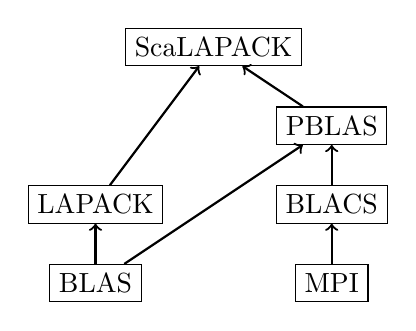
\begin{tikzpicture}
      \node at (0,0) [rectangle,draw] (blas1) {BLAS};
      \node at (0,1) [rectangle,draw] (lapack1) {LAPACK};
      \node at (3,0) [rectangle,draw] (mpi1) {MPI};
      \node at (3,1) [rectangle,draw] (blacs1) {BLACS};
      \node at (3,2) [rectangle,draw] (pblas1) {PBLAS};
      \node at (1.5,3) [rectangle,draw] (scal1) {ScaLAPACK};
      \draw [thick,->] (blas1) -- (lapack1);
      \draw [thick,->] (lapack1) -- (scal1);
      \draw [thick,->] (blas1) -- (pblas1);
      \draw [thick,->] (mpi1) -- (blacs1);
      \draw [thick,->] (blacs1) -- (pblas1);
      \draw [thick,->] (pblas1) -- (scal1);
    \end{tikzpicture}
  \end{center}
  
  \vspace{5mm}
  ScaLAPACK builds additional layers on same idea.

\end{frame}


\begin{frame}
  \frametitle{Reminder: Evolution of LU}

  On board...
\end{frame}


\begin{frame}
  \frametitle{Blocked GEPP}
  
  \begin{center}
    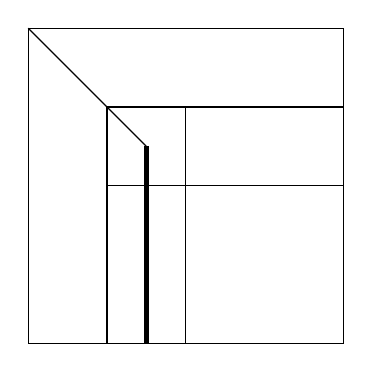
\begin{tikzpicture}
      \draw (0,4) rectangle (4,0);
      \draw (1,3) rectangle (4,0);
      \draw (2,2) rectangle (4,0);
      \draw (1,3) rectangle (2,2);
      \draw (0,4) -- (1.5,2.5);
      \draw[ultra thick] (1.5,2.5) -- (1.5,0);
    \end{tikzpicture}
    
    Find pivot
  \end{center}
\end{frame}


\begin{frame}
  \frametitle{Blocked GEPP}
  
  \begin{center}
    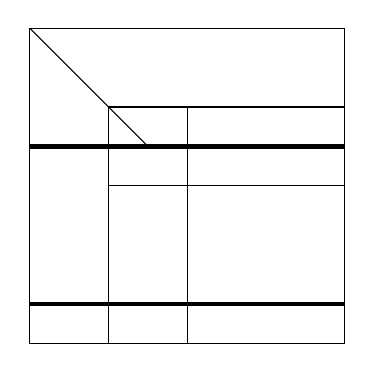
\begin{tikzpicture}
      \draw (0,4) rectangle (4,0);
      \draw (1,3) rectangle (4,0);
      \draw (2,2) rectangle (4,0);
      \draw (1,3) rectangle (2,2);
      \draw (0,4) -- (1.5,2.5);
      \draw[ultra thick] (0,2.5) -- (4,2.5);
      \draw[ultra thick] (0,0.5) -- (4,0.5);
    \end{tikzpicture}
    
    Swap pivot row
  \end{center}

\end{frame}


\begin{frame}
  \frametitle{Blocked GEPP}
  
  \begin{center}
    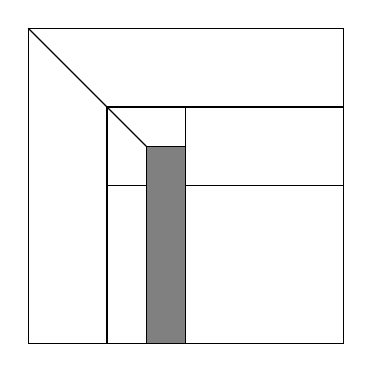
\begin{tikzpicture}
      \draw (0,4) rectangle (4,0);
      \draw (1,3) rectangle (4,0);
      \draw (2,2) rectangle (4,0);
      \draw (1,3) rectangle (2,2);
      \draw (0,4) -- (1.5,2.5);
      \draw[fill=black!50] (1.5,2.5) rectangle (2,0);
    \end{tikzpicture}
    
    Update within block column
  \end{center}
\end{frame}


\begin{frame}
  \frametitle{Blocked GEPP}

  \begin{center}
    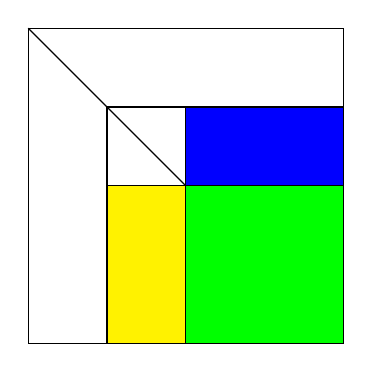
\begin{tikzpicture}
      \draw (0,4) rectangle (4,0);
      \draw (1,3) rectangle (4,0);
      \draw (2,2) rectangle (4,0);
      \draw (1,3) rectangle (2,2);
      \draw (0,4) -- (2,2);
      \draw[fill=yellow] (1,2) rectangle (2,0);
      \draw[fill=blue] (2,3) rectangle (4,2);
      \draw[fill=green] (2,2) rectangle (4,0);
    \end{tikzpicture}
    
    Delayed update (at end of block)
  \end{center}  
\end{frame}


\begin{frame}
  \frametitle{Big idea}
  
  \begin{itemize}
  \item {\em Delayed update} strategy lets us do LU fast
    \begin{itemize}
    \item Could have also delayed application of pivots
    \end{itemize}
  \item Same idea with other one-sided factorizations (QR)
  \item Can get decent multi-core speedup with parallel BLAS! \\
    ... assuming $n$ sufficiently large.
  \end{itemize}
  There are still some issues left over (block size? pivoting?)...
\end{frame}

\begin{frame}
  \frametitle{Explicit parallelization of GE}

  What to do:
  \begin{itemize}
  \item {\em Decompose} into work chunks
  \item {\em Assign} work to threads in a balanced way
  \item {\em Orchestrate} the communication and synchronization
  \item {\em Map} which processors execute which threads
  \end{itemize}
\end{frame}


\begin{frame}
  \frametitle{Possible matrix layouts}

  1D column blocked: bad load balance
  \[
  \begin{bmatrix}
    0 & 0 & 0 & 1 & 1 & 1 & 2 & 2 & 2 \\
    0 & 0 & 0 & 1 & 1 & 1 & 2 & 2 & 2 \\
    0 & 0 & 0 & 1 & 1 & 1 & 2 & 2 & 2 \\
    0 & 0 & 0 & 1 & 1 & 1 & 2 & 2 & 2 \\
    0 & 0 & 0 & 1 & 1 & 1 & 2 & 2 & 2 \\
    0 & 0 & 0 & 1 & 1 & 1 & 2 & 2 & 2 \\
    0 & 0 & 0 & 1 & 1 & 1 & 2 & 2 & 2 \\
    0 & 0 & 0 & 1 & 1 & 1 & 2 & 2 & 2 \\
    0 & 0 & 0 & 1 & 1 & 1 & 2 & 2 & 2 
  \end{bmatrix}
  \]
\end{frame}


\begin{frame}
  \frametitle{Possible matrix layouts}

  1D column cyclic: hard to use BLAS2/3
  \[
  \begin{bmatrix}
    0 & 1 & 2 & 0 & 1 & 2 & 0 & 1 & 2 \\
    0 & 1 & 2 & 0 & 1 & 2 & 0 & 1 & 2 \\
    0 & 1 & 2 & 0 & 1 & 2 & 0 & 1 & 2 \\
    0 & 1 & 2 & 0 & 1 & 2 & 0 & 1 & 2 \\
    0 & 1 & 2 & 0 & 1 & 2 & 0 & 1 & 2 \\
    0 & 1 & 2 & 0 & 1 & 2 & 0 & 1 & 2 \\
    0 & 1 & 2 & 0 & 1 & 2 & 0 & 1 & 2 \\
    0 & 1 & 2 & 0 & 1 & 2 & 0 & 1 & 2 \\
    0 & 1 & 2 & 0 & 1 & 2 & 0 & 1 & 2 
  \end{bmatrix}
  \]
\end{frame}


\begin{frame}
  \frametitle{Possible matrix layouts}

  1D column block cyclic: block column factorization a bottleneck
  \[
  \begin{bmatrix}
    0 & 0 & 1 & 1 & 2 & 2 & 0 & 0 & 1 & 1 \\
    0 & 0 & 1 & 1 & 2 & 2 & 0 & 0 & 1 & 1 \\
    0 & 0 & 1 & 1 & 2 & 2 & 0 & 0 & 1 & 1 \\
    0 & 0 & 1 & 1 & 2 & 2 & 0 & 0 & 1 & 1 \\
    0 & 0 & 1 & 1 & 2 & 2 & 0 & 0 & 1 & 1 \\
    0 & 0 & 1 & 1 & 2 & 2 & 0 & 0 & 1 & 1 \\
    0 & 0 & 1 & 1 & 2 & 2 & 0 & 0 & 1 & 1 \\
    0 & 0 & 1 & 1 & 2 & 2 & 0 & 0 & 1 & 1 \\
    0 & 0 & 1 & 1 & 2 & 2 & 0 & 0 & 1 & 1 \\
    0 & 0 & 1 & 1 & 2 & 2 & 0 & 0 & 1 & 1
  \end{bmatrix}
  \]
\end{frame}


\begin{frame}
  \frametitle{Possible matrix layouts}

  Block skewed: indexing gets messy
  \[
  \begin{bmatrix}
    0 & 0 & 0 & 1 & 1 & 1 & 2 & 2 & 2 \\
    0 & 0 & 0 & 1 & 1 & 1 & 2 & 2 & 2 \\
    0 & 0 & 0 & 1 & 1 & 1 & 2 & 2 & 2 \\
    2 & 2 & 2 & 0 & 0 & 0 & 1 & 1 & 1 \\
    2 & 2 & 2 & 0 & 0 & 0 & 1 & 1 & 1 \\
    2 & 2 & 2 & 0 & 0 & 0 & 1 & 1 & 1 \\
    1 & 1 & 1 & 2 & 2 & 2 & 0 & 0 & 0 \\
    1 & 1 & 1 & 2 & 2 & 2 & 0 & 0 & 0 \\
    1 & 1 & 1 & 2 & 2 & 2 & 0 & 0 & 0 
  \end{bmatrix}
  \]
\end{frame}


\begin{frame}
  \frametitle{Possible matrix layouts}

  2D block cyclic:
  \[
  \begin{bmatrix}
    0 & 0 & 1 & 1 & 0 & 0 & 1 & 1 \\
    0 & 0 & 1 & 1 & 0 & 0 & 1 & 1 \\
    2 & 2 & 3 & 3 & 2 & 2 & 3 & 3 \\
    2 & 2 & 3 & 3 & 2 & 2 & 3 & 3 \\
    0 & 0 & 1 & 1 & 0 & 0 & 1 & 1 \\
    0 & 0 & 1 & 1 & 0 & 0 & 1 & 1 \\
    2 & 2 & 3 & 3 & 2 & 2 & 3 & 3 \\
    2 & 2 & 3 & 3 & 2 & 2 & 3 & 3 \\
  \end{bmatrix}
  \]
\end{frame}



\begin{frame}
  \frametitle{Possible matrix layouts}

  \begin{itemize}
  \item 1D column blocked: bad load balance
  \item 1D column cyclic: hard to use BLAS2/3
  \item 1D column block cyclic: factoring column is a bottleneck
  \item Block skewed (a la Cannon): just complicated
  \item 2D row/column block: bad load balance
  \item 2D row/column block cyclic: win!
  \end{itemize}
\end{frame}


\begin{frame}
  \frametitle{Distributed GEPP}

  \begin{center}
    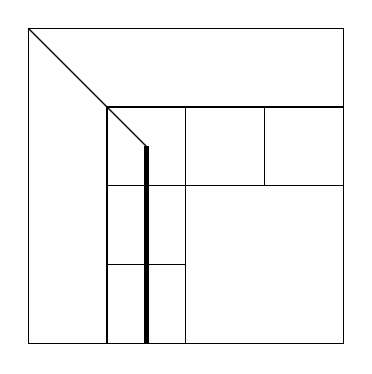
\begin{tikzpicture}
      \draw (0,4) rectangle (4,0);
      \draw (1,3) rectangle (2,2);
      \draw (2,3) rectangle (3,2);
      \draw (3,3) rectangle (4,2);
      \draw (1,2) rectangle (2,1);
      \draw (1,1) rectangle (2,0);
      \draw (0,4) -- (1.5,2.5);
      \draw[ultra thick] (1.5,2.5) -- (1.5,0);
    \end{tikzpicture}

    Find pivot (column broadcast)
  \end{center}
\end{frame}


\begin{frame}
  \frametitle{Distributed GEPP}
  
  \begin{center}
    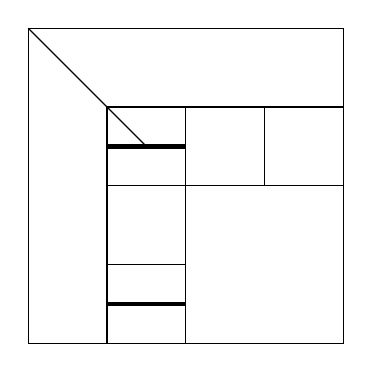
\begin{tikzpicture}
      \draw (0,4) rectangle (4,0);
      \draw (1,3) rectangle (2,2);
      \draw (2,3) rectangle (3,2);
      \draw (3,3) rectangle (4,2);
      \draw (1,2) rectangle (2,1);
      \draw (1,1) rectangle (2,0);
      \draw (0,4) -- (1.5,2.5);
      \draw[ultra thick] (1,2.5) -- (2,2.5);
      \draw[ultra thick] (1,0.5) -- (2,0.5);
    \end{tikzpicture}

    Swap pivot row within block column + 
    broadcast pivot
  \end{center}
\end{frame}


\begin{frame}
  \frametitle{Distributed GEPP}
  
  \begin{center}
    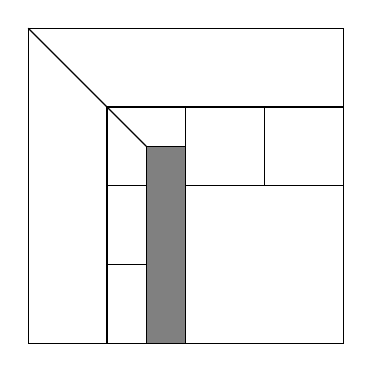
\begin{tikzpicture}
      \draw (0,4) rectangle (4,0);
      \draw (1,3) rectangle (2,2);
      \draw (2,3) rectangle (3,2);
      \draw (3,3) rectangle (4,2);
      \draw (1,2) rectangle (2,1);
      \draw (1,1) rectangle (2,0);
      \draw (0,4) -- (1.5,2.5);
      \draw[fill=black!50] (1.5,2.5) rectangle (2,0);
    \end{tikzpicture}

    Update within block column
  \end{center}
\end{frame}


\begin{frame}
  \frametitle{Distributed GEPP}
  
  \begin{center}
    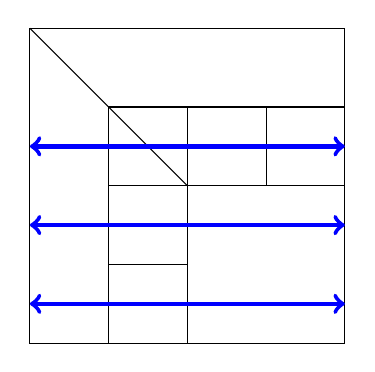
\begin{tikzpicture}
      \draw (0,4) rectangle (4,0);
      \draw (1,3) rectangle (2,2);
      \draw (2,3) rectangle (3,2);
      \draw (3,3) rectangle (4,2);
      \draw (1,2) rectangle (2,1);
      \draw (1,1) rectangle (2,0);
      \draw (0,4) -- (2,2);
      \draw[ultra thick, blue, <->] (0,2.5) -- (4,2.5);
      \draw[ultra thick, blue, <->] (0,1.5) -- (4,1.5);
      \draw[ultra thick, blue, <->] (0,0.5) -- (4,0.5);
    \end{tikzpicture}

    At end of block, broadcast swap info along rows
  \end{center}
\end{frame}


\begin{frame}
  \frametitle{Distributed GEPP}
  
  \begin{center}
    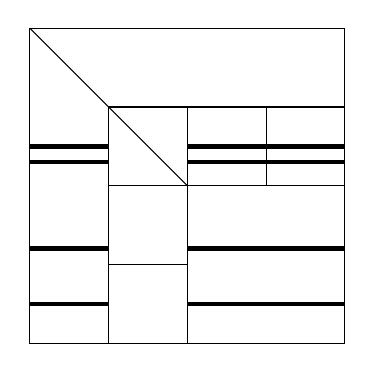
\begin{tikzpicture}
      \draw (0,4) rectangle (4,0);
      \draw (1,3) rectangle (2,2);
      \draw (2,3) rectangle (3,2);
      \draw (3,3) rectangle (4,2);
      \draw (1,2) rectangle (2,1);
      \draw (1,1) rectangle (2,0);
      \draw (0,4) -- (2,2);
      \draw[ultra thick] (0,2.5) -- (1,2.5);
      \draw[ultra thick] (0,2.3) -- (1,2.3);
      \draw[ultra thick] (0,0.5) -- (1,0.5);
      \draw[ultra thick] (0,1.2) -- (1,1.2);
      \draw[ultra thick] (2,2.5) -- (4,2.5);
      \draw[ultra thick] (2,2.3) -- (4,2.3);
      \draw[ultra thick] (2,0.5) -- (4,0.5);
      \draw[ultra thick] (2,1.2) -- (4,1.2);
    \end{tikzpicture}

    Apply all row swaps to other columns
  \end{center}
\end{frame}


\begin{frame}
  \frametitle{Distributed GEPP}
  
  \begin{center}
    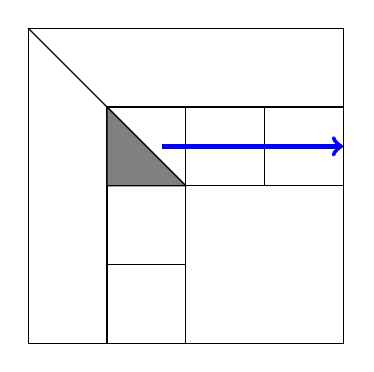
\begin{tikzpicture}
      \draw (0,4) rectangle (4,0);
      \draw (1,3) rectangle (2,2);
      \draw (2,3) rectangle (3,2);
      \draw (3,3) rectangle (4,2);
      \draw (1,2) rectangle (2,1);
      \draw (1,1) rectangle (2,0);
      \draw (0,4) -- (2,2);
      \draw [fill=black!50] (1,3) -- (2,2) -- (1,2) -- cycle;
      \draw [ultra thick,blue,->] (1.7,2.5) -- (4,2.5);
    \end{tikzpicture}
    
    Broadcast block $L_{II}$ right
  \end{center}
\end{frame}


\begin{frame}
  \frametitle{Distributed GEPP}
  
  \begin{center}
    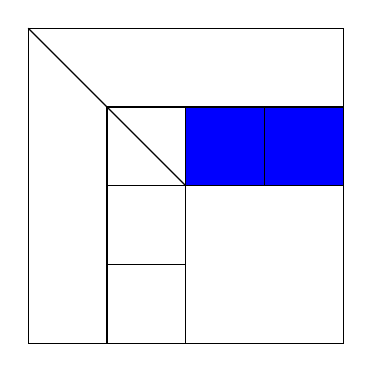
\begin{tikzpicture}
      \draw [fill=blue] (2,3) rectangle (4,2);
      \draw (0,4) rectangle (4,0);
      \draw (1,3) rectangle (2,2);
      \draw (2,3) rectangle (3,2);
      \draw (3,3) rectangle (4,2);
      \draw (1,2) rectangle (2,1);
      \draw (1,1) rectangle (2,0);
      \draw (0,4) -- (2,2);
    \end{tikzpicture}
    
    Update remainder of block row
  \end{center}
\end{frame}


\begin{frame}
  \frametitle{Distributed GEPP}
  
  \begin{center}
    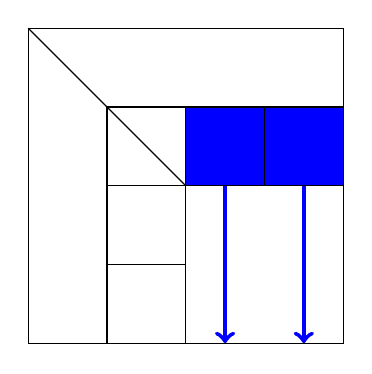
\begin{tikzpicture}
      \draw [fill=blue] (2,3) rectangle (4,2);
      \draw (0,4) rectangle (4,0);
      \draw (1,3) rectangle (2,2);
      \draw (2,3) rectangle (3,2);
      \draw (3,3) rectangle (4,2);
      \draw (1,2) rectangle (2,1);
      \draw (1,1) rectangle (2,0);
      \draw (0,4) -- (2,2);
      \draw[ultra thick,blue,->] (2.5,2) -- (2.5,0);
      \draw[ultra thick,blue,->] (3.5,2) -- (3.5,0);
    \end{tikzpicture}
    
    Broadcast rest of block row down
  \end{center}
\end{frame}


\begin{frame}
  \frametitle{Distributed GEPP}
  
  \begin{center}
    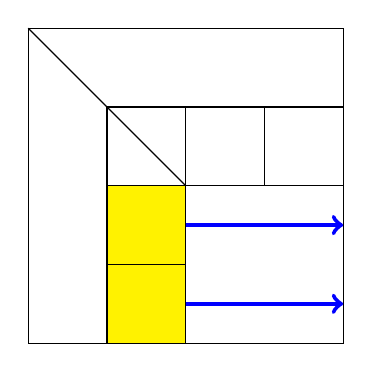
\begin{tikzpicture}
      \draw [fill=yellow] (1,2) rectangle (2,0);
      \draw (0,4) rectangle (4,0);
      \draw (1,3) rectangle (2,2);
      \draw (2,3) rectangle (3,2);
      \draw (3,3) rectangle (4,2);
      \draw (1,2) rectangle (2,1);
      \draw (1,1) rectangle (2,0);
      \draw (0,4) -- (2,2);
      \draw[ultra thick,blue,->] (2,1.5) -- (4,1.5);
      \draw[ultra thick,blue,->] (2,0.5) -- (4,0.5);
    \end{tikzpicture}
  
    Broadcast rest of block col right
  \end{center}
\end{frame}


\begin{frame}
  \frametitle{Distributed GEPP}
  
  \begin{center}
    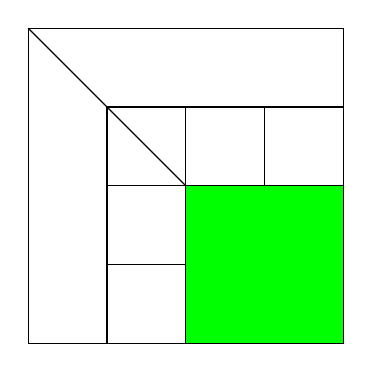
\begin{tikzpicture}
      \draw [fill=green] (2,2) rectangle (4,0);
      \draw (0,4) rectangle (4,0);
      \draw (1,3) rectangle (2,2);
      \draw (2,3) rectangle (3,2);
      \draw (3,3) rectangle (4,2);
      \draw (1,2) rectangle (2,1);
      \draw (1,1) rectangle (2,0);
      \draw (0,4) -- (2,2);
    \end{tikzpicture}
  
    Update of trailing submatrix
  \end{center}
\end{frame}


\begin{frame}
  \frametitle{Cost of ScaLAPACK GEPP}
  
  Communication costs:
  \begin{itemize}
  \item Lower bound: $O(n^2/\sqrt{P})$ words, $O(\sqrt{P})$ messages
  \item ScaLAPACK: 
    \begin{itemize}
    \item $O(n^2 \log P / \sqrt{P})$ words sent
    \item {\color{red} $O(n \log p)$} messages
    \item Problem: reduction to find pivot in each column
    \end{itemize}
  \item Recent research on stable variants without partial pivoting
  \end{itemize}
\end{frame}


\begin{frame}
  \begin{center}
  What if you don't care about dense Gaussian elimination? \\
  Let's review some ideas in a different setting...
  \end{center}
\end{frame}


\begin{frame}
  \frametitle{Floyd-Warshall}
  
  Goal: Find shortest path lengths between all node pairs. \\[5mm]
  Idea: Dynamic programming!  Define
  \[
    d_{ij}^{(k)} =
    \mbox{shortest path $i$ to $j$ with intermediates in $\{1, \ldots, k\}$}.
  \]
  Then
  \[
    d_{ij}^{(k)} = 
    \min\left( d_{ij}^{(k-1)}, d_{ik}^{(k-1)} + d_{kj}^{(k-1)} \right)
  \]
  and $d_{ij}^{(n)}$ is the desired shortest path length.
\end{frame}


\begin{frame}[fragile]
  \frametitle{The same and different}

Floyd's algorithm for all-pairs shortest paths:
\begin{lstlisting}
for k=1:n
  for i = 1:n
    for j = 1:n
      D(i,j) = min(D(i,j), D(i,k)+D(k,j));
\end{lstlisting}

\vspace{5mm}
Unpivoted Gaussian elimination (overwriting $A$):
\begin{lstlisting}
for k=1:n
  for i = k+1:n
    A(i,k) = A(i,k) / A(k,k);
    for j = k+1:n
      A(i,j) = A(i,j)-A(i,k)*A(k,j);
\end{lstlisting}

\end{frame}


\begin{frame}
  \frametitle{The same and different}
  
  \begin{itemize}
  \item The same: $O(n^3)$ time, $O(n^2)$ space
  \item The same: can't move $k$ loop (data dependencies)
    \begin{itemize}
    \item ... at least, can't without care!
    \item Different from matrix multiplication
    \end{itemize}
  \item The same: 
    $x_{ij}^{(k)} = f\left(x_{ij}^{(k-1)}, 
    g\left(x_{ik}^{(k-1)}, x_{kj}^{(k-1)}\right)\right)$
    \begin{itemize}
    \item Same basic dependency pattern in updates!
    \item Similar algebraic relations satisfied
    \end{itemize}
  \item Different: Update to full matrix vs trailing submatrix
  \end{itemize}
\end{frame}


\begin{frame}
  \frametitle{How far can we get?}
  
  How would we
  \begin{itemize}
  \item Write a cache-efficient (blocked) {\em serial} implementation?
  \item Write a message-passing {\em parallel} implementation?
  \end{itemize}

  \vspace{1cm}
  The full picture could make a fun class project...

\end{frame}


\begin{frame}
  \frametitle{Onward!}
  
  Next up: Sparse linear algebra and iterative solvers!
\end{frame}

\end{document}
